\section{Registers}

The processor has sixteen 32 bit registers. Four of the 32 bit registers are divided into sixteen 8 bit registers and eight of the
32 bit registers are divided into sixteen 16 bit registers. Additionally the processor has sixteen 32 bit control registers.

\begin{figure}[H]
\begin{center}
	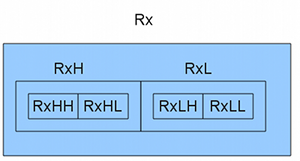
\includegraphics{./files/regdiv.png}
\end{center}
	\caption{Division of 32 bit register into 8 bit/16 bit registers}
\end{figure}

Example:
The R0 register is 32 bit register and is devided into two 16 bit and four 8 bit registers.
\begin{description}
\item[dword register] R0
\item[word registers] R0L, R0H
\item[byte registers] R0LL, R0LH, R0HL, R0HH
\end{description}

\subsection{Instruction Pointer}

The Instruction Pointer (IP) is a hidden register and can only be accessed through \verb|JMP|-/\verb|CALL|-Instructions or stack manipulation
inside Interrupt Service Routines (see section~\elref{sec:interrupts}). The
Instruction Pointer always points to the next instruction. If the Instruction Pointer overflows (or underflows) its value will be undefined.
You must not assume that the Instruction Pointer wraps around. 

\subsection{Control registers}

\begin{tabular}{ | c | l | }
	\hline                        
	\textbf{Mnemonic} & \textbf{Description} \\
	\hline
	MR1 & Holds the address of the page directory\\
	\hline
	MR2 & Holds MMU control flags \\
	\hline
	MR3 & Virtual Address Register \\
	\hline
	MR4 & Error Code Register \\
	\hline
	CR1 & Holds control flags \\
	\hline
	CR2 & Reserved \\
	\hline
	SSP & System stack pointer \\
	\hline
        ST1 & Storage Register 1. Intended for use by an operating system as a temporary storage. \\
	\hline
	ST2 & Storage Register 2. Intended for use by an operating system as a temporary storage. \\
	\hline
	ST3 & Storage Register 3. Intended for use by an operating system as a temporary storage. \\
	\hline
	ST4 & Storage Register 4. Intended for use by an operating system as a temporary storage. \\
	\hline
\end{tabular}

\subsubsection{SSP}

The system stack pointer is used by the CPU when handling interrupts. Handling interrupts requires to reading/writing values to/from the stack. 
When handling interrupts the CPU uses the SSP register as the stack pointer instead of the regular SP. 

\subsubsection{MR2 Flags}

\begin{tabular}{| r | r |}
	\hline
	Reserved [31] & MMU Enabled \\
	\hline
\end{tabular}

\begin{itemize}
	\item MMU Enabled - If this flag is set paging is enabled. 
\end{itemize}

\subsubsection{CR1 Flags}

\begin{tabular}{ | r | r | r | r | r | }
	\hline
	Reserved [28] & FAILURE & EXCEPTION & PRIV\_MODE & INT\_ENABLED \\
	\hline
\end{tabular}

\begin{itemize}
	\item FAILURE - Failure Flag : This flag is set by the CPU when an exception occurs and the Exception Flag is set
	\item EXCEPTION - Exception Flag : This flag is set by the CPU when calling an exception (ISR). 
	\item PRIV\_MODE - Privileged Mode Flag : If this flag is set the CPU is in privileged mode (otherwise the CPU is in unprivileged mode).
	\item INT\_ENABLED - Interrupts Enabled : If this flag is set the CPU will handle hardware interrupts. 
\end{itemize}

It is technically possible to circumvent the double/triple fault mechanism of the CPU. Since this is not recommended it is not further documented how to do this
in this documentation.

\subsection{32 bit}

\begin{tabular}{ | c | l | }
	\hline                        
	\textbf{Mnemonic} & \textbf{Description} \\
	\hline
	R0 & General purpose register \\
	\hline
	R1 & General purpose register \\
	\hline
	R2 & General purpose register \\
	\hline
	R3 & General purpose register \\
	\hline
	R4 & General purpose register \\
	\hline
	R5 & General purpose register \\
	\hline
	R6 & General purpose register \\
	\hline
	R7 & General purpose register \\
	\hline
	R8 & General purpose register \\
	\hline
	R9 & General purpose register \\
	\hline
	RA & General purpose register \\
	\hline
	RB & General purpose register \\
	\hline
	RC & Return address register \\
	\hline
	BP & Base pointer register \\
	\hline
	SP & Stack pointer register \\
	\hline
	FLGS & Flags register \\
	\hline
\end{tabular}

\subsubsection{FLGS flags}

\begin{tabular}{ | r | r | r | r | r | r | r | }
	\hline
	Reserved [26] & E & S & P & O & C & Z	\\
	\hline
\end{tabular}

\begin{itemize}
	\item E - Even Flag
	\item S - Sign Flag
	\item P - Parity Flag
	\item O - Overflow Flag
	\item C - Carry Flag
	\item Z - Zero Flag
\end{itemize}

\subsection{16 bit}

\begin{tabular}{ | c | l | }
	\hline                        
	\textbf{Mnemonic} & \textbf{Description} \\
	\hline
	R0L & General purpose register \\
	\hline
	R0H & General purpose register \\
	\hline
	R1L & General purpose register \\
	\hline
	R1H & General purpose register \\
	\hline
	R2L & General purpose register \\
	\hline
	R2H & General purpose register \\
	\hline
	R3L & General purpose register \\
	\hline
	R3H & General purpose register \\
	\hline
	R4L & General purpose register \\
	\hline
	R4H & General purpose register \\
	\hline
	R5L & General purpose register \\
	\hline
	R5H & General purpose register \\
	\hline
	R6L & General purpose register \\
	\hline
	R6H & General purpose register \\
	\hline
	R7L & General purpose register \\
	\hline
	R7H & General purpose register \\
	\hline
\end{tabular}

\subsection{8 bit}

\begin{tabular}{ | c | l | }
	\hline                        
	\textbf{Mnemonic} & \textbf{Description} \\
	\hline
	R0LL & General purpose register \\
	\hline
	R0LH & General purpose register \\
	\hline
	R0HL & General purpose register \\
	\hline
	R0HH & General purpose register \\
	\hline
	R1LL & General purpose register \\
	\hline
	R1LH & General purpose register \\
	\hline
	R1HL & General purpose register \\
	\hline
	R1HH & General purpose register \\
	\hline
	R2LL & General purpose register \\
	\hline
	R2LH & General purpose register \\
	\hline
	R2HL & General purpose register \\
	\hline
	R2HH & General purpose register \\
	\hline
	R3LL & Return address register \\
	\hline
	R3LH & General purpose register \\
	\hline
	R3HL & General purpose register \\
	\hline
	R3HH & General purpose register \\
	\hline
\end{tabular}

\subsection{Initial values}

The initial values of all general purpose registers are undefined. The initial values of SSP, MR1, MR3 and MR4 are undefined as well.
CR1 is initialized with only the Privileged Mode Flag set. MR2 is initialized to zero. 
